%% Included in decks: slidemage-manual, slidemage-manual-copy
%%

% SlideMage manual, chapter "Working in SlideMage": the deck editor, showing
% this manual's own deck (tools/manual/make_screenshots.py).
\setSlideVersion{1-0-0}
\providecommand{\callout}[2]{\node[circle, fill=c_primary_highlight, text=white, inner sep=1pt, minimum size=9pt, font=\tiny\bfseries] at (#1) {#2};}
\begin{standardframe}{The deck editor}
	\small
	Click a deck's name in the main window to open the deck editor: one row per slide and per chapter, in deck order. Everything you do here -- adding, moving,	removing slides and chapters -- is written into the deck file at once (with an \emph{Undo} option), so you never need to edit it by hand.
	\par\smallskip
	\begingroup\centering
		\begin{tikzpicture}
			\node[anchor=south west, inner sep=0pt] (shot) at (0,0) {\setlength{\fboxsep}{0pt}\setlength{\fboxrule}{0.4pt}\fcolorbox{c_primary_gray}{white}{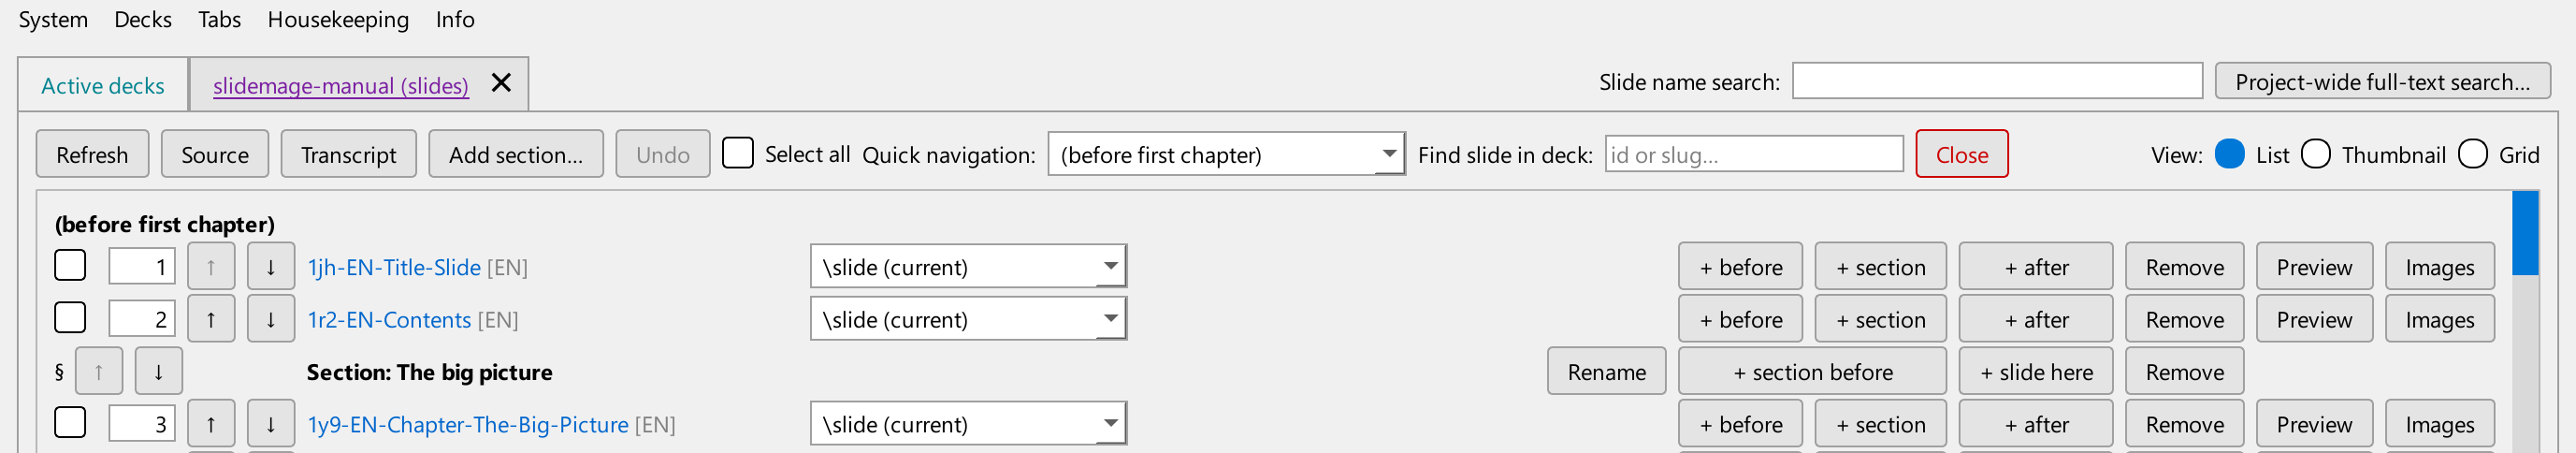
\includegraphics[width=0.88\linewidth]{media/screenshot-slidemage-deck-editor-list.png}}};
			\begin{scope}[x={(shot.south east)}, y={(shot.north west)}]
				% beside each element (tools/manual/make_screenshots.py prints the
				% elements' centres; the picture is the top of the list, 2754 x 502 px)
						\callout{0.235,0.795}{1}
						\callout{0.476,0.795}{2}
						\callout{0.806,0.673}{3}
						\callout{0.016,0.495}{4}
						\callout{0.078,0.495}{5}
						\callout{0.255,0.434}{6}
						\callout{0.465,0.434}{7}
						\callout{0.633,0.434}{8}
						\callout{0.88,0.55}{9}
						\callout{0.585,0.211}{10}
			\end{scope}
		\end{tikzpicture}
	\par\endgroup
	\vspace{-4pt}
	\begin{columns}[T,onlytextwidth]
		\begin{column}{0.49\linewidth}
			\scriptsize
			\begin{enumerate}
				\item Toolbar: refresh, source, transcript, add section, undo
				\item \emph{Quick navigation}; \emph{Find slide in deck}
				\item View: \emph{List}, \emph{Thumbnail} or \emph{Grid}
				\item Tick slides to remove several at once
				\item Move a slide: type a number or use the arrows
			\end{enumerate}
		\end{column}
		\begin{column}{0.49\linewidth}
			\scriptsize
			\begin{enumerate}
				\setcounter{enumi}{5}
				\item Click a slide's ID to open it in the slide editor
				\item Dropdown: how the slide is included (\SMCmd{slide} \ldots)
				\item \emph{+ before}, \emph{+ section}, \emph{+ after}: add a slide or section here
				\item \emph{Remove}, \emph{Preview}, \emph{Images} of this slide
				\item Section row: move, rename, add, remove
			\end{enumerate}
		\end{column}
	\end{columns}
\end{standardframe}
